
\section{Examples}
\label{examples}
\subsection{CompartmentGlyph Example}
Below a \CompartmentGlyph is defined for the compartment \token{Yeast}. 
It is located at position \token{x=5, y=5} and has dimensions 
\token{width=390, height=220}. 

\label{example:compartmentglyph}
\paragraph{\sbmlthreecore using the \LayoutPackage}
\begin{example}
<?xml version="1.0" encoding="UTF-8"?>
<sbml xmlns="http://www.sbml.org/sbml/level3/version1/core" 
		xmlns:layout="http://www.sbml.org/sbml/level3/version1/layout/version1" 
		level="3" version="1" layout:required="false" >		
  <model id="TestModel_with_modifiers">
                .
                .
                .
    <listOfCompartments>
      <compartment id="Yeast" spatialDimensions="3" constant="true"/>
    </listOfCompartments>	
                .
                .
                .
    <layout:listOfLayouts xmlns:xsi="http://www.w3.org/2001/XMLSchema-instance" 
		xmlns:layout="http://www.sbml.org/sbml/level3/version1/layout/version1">
      <layout:layout layout:id="Layout_1">
        <layout:dimensions layout:width="400" layout:height="230"/>
        <layout:listOfCompartmentGlyphs>
          <layout:compartmentGlyph layout:id="CompartmentGlyph_1" layout:compartment="Yeast">
            <layout:boundingBox layout:id="bb1">
              <layout:position layout:x="5" layout:y="5"/>
              <layout:dimensions layout:width="390" layout:height="220"/>
            </layout:boundingBox>
          </layout:compartmentGlyph>
        </layout:listOfCompartmentGlyphs>
                .
                .
                .
			</layout:layout>
		</layout:listOfLayouts>
  </model>
</sbml>
\end{example}
\paragraph{SBML Level~2 Version~1 using the Annotation Scheme}
\begin{example}
<?xml version="1.0" encoding="UTF-8"?>
<sbml xmlns="http://www.sbml.org/sbml/level2" level="2" version="1">
  <model id="TestModel_with_modifiers">
    <annotation>
     <listOfLayouts xmlns="http://projects.eml.org/bcb/sbml/level2"
              xmlns:xsi="http://www.w3.org/2001/XMLSchema-instance">
      <layout id="Layout_1">
        <dimensions width="400" height="230"/>
        <listOfCompartmentGlyphs>
          <compartmentGlyph id="CompartmentGlyph_1" compartment="Yeast">
            <boundingBox id="bb1">
              <position x="5" y="5"/>
              <dimensions width="390" height="220"/>
            </boundingBox>
          </compartmentGlyph>
        </listOfCompartmentGlyphs>
                .
                .
                .
      </layout>
     </listOfLayouts>
    </annotation>
    <listOfCompartments>
      <compartment id="Yeast"/>
    </listOfCompartments>
        .
        .
        .
  </model> 
</sbml>
\end{example}

\subsection{SpeciesGlyph Example}
Below a \SpeciesGlyph is defined for the species \token{Glucose} at 
position \token{x=105, y=20} with dimensions \token{width=130, 
height=20}. 

\label{example:speciesglyph}
\paragraph{\sbmlthreecore using the \LayoutPackage}
\begin{example}
<?xml version="1.0" encoding="UTF-8"?>
<sbml xmlns="http://www.sbml.org/sbml/level3/version1/core" 
		xmlns:layout="http://www.sbml.org/sbml/level3/version1/layout/version1" 
		level="3" version="1" layout:required="false" >		
  <model id="TestModel_with_modifiers">
                .
                .
                .
    <listOfSpecies>
      <species id="Glucose" compartment="Yeast" substanceUnits="substance" 
			hasOnlySubstanceUnits="false" boundaryCondition="false" constant="false"/>
    </listOfSpecies>
                .
                .
                .
    <layout:listOfLayouts xmlns:xsi="http://www.w3.org/2001/XMLSchema-instance" 
		xmlns:layout="http://www.sbml.org/sbml/level3/version1/layout/version1">
      <layout:layout layout:id="Layout_1">
        <layout:dimensions layout:width="400" layout:height="230"/>
                .
                .
                .
        <layout:listOfSpeciesGlyphs>
          <layout:speciesGlyph layout:id="SpeciesGlyph_Glucose"  layout:species="Glucose">
            <layout:boundingBox layout:id="bb2">
              <layout:position layout:x="105" layout:y="20"/>
              <layout:dimensions layout:width="130" layout:height="20"/>
            </layout:boundingBox>
          </layout:speciesGlyph>
        </layout:listOfSpeciesGlyphs>					
                .
                .
                .
			</layout:layout>
		</layout:listOfLayouts>
  </model>
</sbml>
\end{example}
\pagebreak
\paragraph{SBML Level~2 Version~1 using the Annotation Scheme}
\begin{example}
<?xml version="1.0" encoding="UTF-8"?>
<sbml xmlns="http://www.sbml.org/sbml/level2" level="2" version="1">
  <model id="TestModel_with_modifiers">
    <annotation>
     <listOfLayouts xmlns="http://projects.eml.org/bcb/sbml/level2"
              xmlns:xsi="http://www.w3.org/2001/XMLSchema-instance">
      <layout id="Layout_1">
        <dimensions width="400" height="230"/>
                .
                .
                .
        <listOfSpeciesGlyphs>
          <speciesGlyph id="SpeciesGlyph_Glucose" species="Glucose">
            <boundingBox id="bb2">
              <position x="105" y="20"/>
              <dimensions width="130" height="20"/>
            </boundingBox>
          </speciesGlyph>
        </listOfSpeciesGlyphs>  
            .
            .
            . 
       </layout>
      </listOfLayouts>
    </annotions>
         .
         .
         .
    <listOfSpecies>
      <species id="Glucose" compartment="Yeast"/>
    </listOfSpecies>
       .
       .
       .  
  </model>
</sbml>
\end{example}


\subsection{ReactionGlyph Example}
The following defines a \ReactionGlyph for reaction \token{Hexokinase} 
containing only a center segment represented as straight line. 

\label{example:reactionglyph}
\paragraph{\sbmlthreecore using the \LayoutPackage}
\begin{example}
<?xml version="1.0" encoding="UTF-8"?>
<sbml xmlns="http://www.sbml.org/sbml/level3/version1/core" 
		xmlns:layout="http://www.sbml.org/sbml/level3/version1/layout/version1" 
		level="3" version="1" layout:required="false" >		
  <model id="TestModel_with_modifiers">
                .
                .
                .
    <listOfReactions>
      <reaction id="Hexokinase" reversible="false" fast="false">
                .
                .
                .
      </reaction
    </listOfReactions>
                .
                .
                .
     <layout:listOfLayouts xmlns:xsi="http://www.w3.org/2001/XMLSchema-instance" 
		xmlns:layout="http://www.sbml.org/sbml/level3/version1/layout/version1">
      <layout:layout layout:id="Layout_1">
        <layout:dimensions layout:width="400" layout:height="230"/>
                .
                .
                .
        <layout:listOfReactionGlyphs>
          <layout:reactionGlyph layout:id="glyph_Hexokinase" layout:reaction="Hexokinase">
            <layout:curve>
              <layout:listOfCurveSegments>
                <layout:curveSegment 
					xmlns:xsi="http://www.w3.org/2001/XMLSchema-instance" 
					xsi:type="LineSegment">
                  <layout:start layout:x="170" layout:y="100"/>
                  <layout:end layout:x="170" layout:y="130"/>
                </layout:curveSegment>
              </layout:listOfCurveSegments>
            </layout:curve>
            <layout:listOfSpeciesReferenceGlyphs>
                .
                .
                .
            </layout:listOfSpeciesReferenceGlyphs>
          </layout:reactionGlyph>
        </layout:listOfReactionGlyphs>
                .
                .
                .
			</layout:layout>
		</layout:listOfLayouts>
  </model>
</sbml>
\end{example}
\paragraph{SBML Level~2 Version~1 using the Annotation Scheme}

\begin{example}
<?xml version="1.0" encoding="UTF-8"?>
<sbml xmlns="http://www.sbml.org/sbml/level2" level="2" version="1">
  <model id="TestModel_with_modifiers">
    <annotation>
     <listOfLayouts xmlns="http://projects.eml.org/bcb/sbml/level2"
              xmlns:xsi="http://www.w3.org/2001/XMLSchema-instance">
      <layout id="Layout_1">
        <dimensions width="400" height="230"/>
              .
              .
              .
        <listOfReactionGlyphs>
          <reactionGlyph id="glyph_Hexokinase" reaction="Hexokinase">
            <curve>
              <listOfCurveSegments>
                <curveSegment xsi:type="LineSegment">
                  <start x="170" y="100"/>
                  <end x="170" y="130"/>
                </curveSegment>
              </listOfCurveSegments>
            </curve>
            <listOfSpeciesReferenceGlyphs>
                    .
                    .
                    .
            </listOfSpeciesReferenceGlyphs>
          </reactionGlyph>
        </listOfReactionGlyphs>
             .
             .
             .
      </layout>
     </listOfLayouts>
    </annotation>
          .
          .
          .
    <listOfReactions>
      <reaction id="Hexokinase" reversible="false">
                    .
                    .
                    .
      </reaction>
    </listOfReactions>  
        .
        .
        .    
  </model>
</sbml>
\end{example}

The following adds a \SpeciesReferenceGlyph and demonstrates adding an 
\token{id} to a \SpeciesReference in SBML Level~2 Version~1. 
This is not necessary in \sbmlthreecore, as there \SpeciesReference
elements have an \token{id} attribute.

\label{example:speciesreferenceid}
\begin{example}
<?xml version="1.0" encoding="UTF-8"?>
<sbml xmlns="http://www.sbml.org/sbml/level2" level="2" version="1">
  <model id="TestModel_with_modifiers">
    <annotation>
     <listOfLayouts xmlns="http://projects.eml.org/bcb/sbml/level2"
              xmlns:xsi="http://www.w3.org/2001/XMLSchema-instance">
      <layout id="Layout_1">
        <dimensions width="400" height="230">
        </dimensions>
              .
              .
              .
        <listOfReactionGlyphs>
          <reactionGlyph id="glyph_Hexokinase" reaction="Hexokinase">
                    .
                    .
                    .
            <listOfSpeciesReferenceGlyphs>
              <speciesReferenceGlyph id="SpeciesReferenceGlyph_Glucose"
                   speciesReference="SpeciesReference_Glucose"
                   speciesGlyph="SpeciesGlyph_Glucose" role="substrate">
                <curve>
                  <listOfCurveSegments>
                    <curveSegment xsi:type="LineSegment">
                      <start x="170" y="100">
                      </start>
                      <end x="170" y="50">
                      </end>
                    </curveSegment>
                  </listOfCurveSegments>
                </curve>
              </speciesReferenceGlyph>
                        .
                        .
                        . 
            </listOfSpeciesReferenceGlyphs>
          </reactionGlyph>
        </listOfReactionGlyphs>
             .
             .
             .
      </layout>
     </listOfLayouts>
    </annotation>
        .
        .
        .
    <listOfReactions>
      <reaction id="Hexokinase" reversible="false">
        <listOfReactants>
          <speciesReference species="Glucose">
            <annotation>
              <layoutId xmlns="http://projects.eml.org/bcb/sbml/level2"
                        id="SpeciesReference_Glucose"/>
            </annotation>
          </speciesReference>
                .
                .
                .
        </listOfReactants>
      </reaction>
    </listOfReactions>
          .
          .
          .  
  </model>
</sbml>
\end{example}


\subsection{TextGlyph Example}
The following defines a \TextGlyph with \token{id=TextGlyph\_Glucose} 
that is connected to a \SpeciesGlyph \\ \token{SpeciesGlyph\_Glucose} 
and retrieves the text to display from the \Species with 
\token{id="Glucose"}. 

\label{example:textglyph}
\paragraph{\sbmlthreecore using the \LayoutPackage}
\begin{example}
<?xml version="1.0" encoding="UTF-8"?>
<sbml xmlns="http://www.sbml.org/sbml/level3/version1/core" 
		xmlns:layout="http://www.sbml.org/sbml/level3/version1/layout/version1" 
		level="3" version="1" layout:required="false" >		
  <model id="TestModel_with_modifiers">
                .
                .
                .
    <listOfSpecies>
      <species id="Glucose" compartment="Yeast" substanceUnits="substance" 
			hasOnlySubstanceUnits="false" boundaryCondition="false" constant="false"/>
    </listOfSpecies>
                .
                .
                .
    <layout:listOfLayouts xmlns:xsi="http://www.w3.org/2001/XMLSchema-instance" 
		xmlns:layout="http://www.sbml.org/sbml/level3/version1/layout/version1">
      <layout:layout layout:id="Layout_1">
        <layout:dimensions layout:width="400" layout:height="230"/>
                .
                .
                .
        <layout:listOfSpeciesGlyphs>
          <layout:speciesGlyph layout:id="SpeciesGlyph_Glucose"  layout:species="Glucose">
            <layout:boundingBox layout:id="bb2">
              <layout:position layout:x="105" layout:y="20"/>
              <layout:dimensions layout:width="130" layout:height="20"/>
            </layout:boundingBox>
          </layout:speciesGlyph>
        </layout:listOfSpeciesGlyphs>					
                .
                .
                .
        <layout:listOfTextGlyphs>
          <layout:textGlyph layout:id="TextGlyph_Glucose" 
			layout:originOfText="Glucose" 
			layout:graphicalObject="SpeciesGlyph_Glucose">
            <layout:boundingBox layout:id="bbA">
              <layout:position layout:x="115" layout:y="20"/>
              <layout:dimensions layout:width="110" layout:height="20"/>
            </layout:boundingBox>
          </layout:textGlyph>
        </layout:listOfTextGlyphs>
                .
                .
                .
			</layout:layout>
		</layout:listOfLayouts>
  </model>
</sbml>
\end{example}
\paragraph{SBML Level~2 Version~1 using the Annotation Scheme}

\begin{example}
<?xml version="1.0" encoding="UTF-8"?>
<sbml xmlns="http://www.sbml.org/sbml/level2" level="2" version="1">
  <model id="TestModel_with_modifiers">
    <annotation>
     <listOfLayouts xmlns="http://projects.eml.org/bcb/sbml/level2"
              xmlns:xsi="http://www.w3.org/2001/XMLSchema-instance">
      <layout id="Layout_1">
        <dimensions width="400" height="230"/>
                .
                .
                .
        <listOfSpeciesGlyphs>
          <speciesGlyph id="SpeciesGlyph_Glucose" species="Glucose">
            <boundingBox id="bb2">
              <position x="105" y="20"/>
              <dimensions width="130" height="20"/>
            </boundingBox>
          </speciesGlyph>
        </listOfSpeciesGlyphs>  
                .
                .
                .
        <listOfTextGlyphs>
          <textGlyph id="TextGlyph_Glucose" graphicalObject="SpeciesGlyph_Glucose"
                     originOfText="Glucose">
            <boundingBox id="bbA">
              <position x="115" y="20">
              </position>
              <dimensions width="110" height="20">
              </dimensions>
            </boundingBox>
          </textGlyph>
        </listOfTextGlyphs>  
            .
            .
            .
      </layout>
     </listOfLayouts>
    </annotation>    
         .
         .
         .
    <listOfSpecies>
      <species id="Glucose" name="Glucose" compartment="Yeast"/>
    </listOfSpecies>
       .
       .
       .  
  </model>
</sbml>
\end{example}

\subsection{Complete Example using SBML Level~3 Version~1}
Here a small complete example to illustrate and complement the 
paragraphs above. The model consists of the Hexokinase reaction. 


\begin{center}
\begin{figure}[h!]
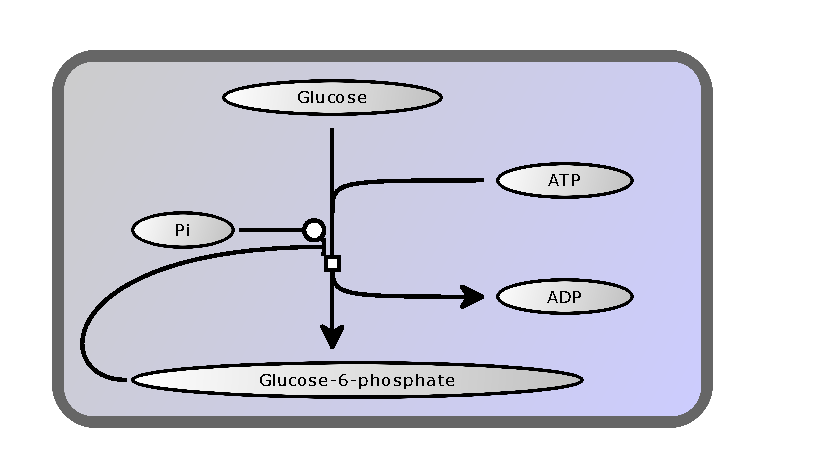
\includegraphics{figures/layout-spec-example}
\caption{One possible rendering of the example layout.}
\end{figure}
\end{center}

This reaction has a feedback inhibition by glucose-6-phosphate and it is 
activated by free organic phosphate. These two relations are represented 
by species reference glyphs and a corresponding role attribute. We did 
not include any coordinates in the third dimension. 

\exampleFile{xml/layout-spec-example-l3v1.xml}
\pagebreak
\subsection{Complete Example using SBML Level~2 Version~1}
\label{l2example}
As mentioned before, the \Layout package has been used since 2003 in 
\SBML Level~2 documents. Whereas the previous example used the Level~3 
package, here we are using the \SBML annotations. 


\begin{center}
\begin{figure}[!ht]
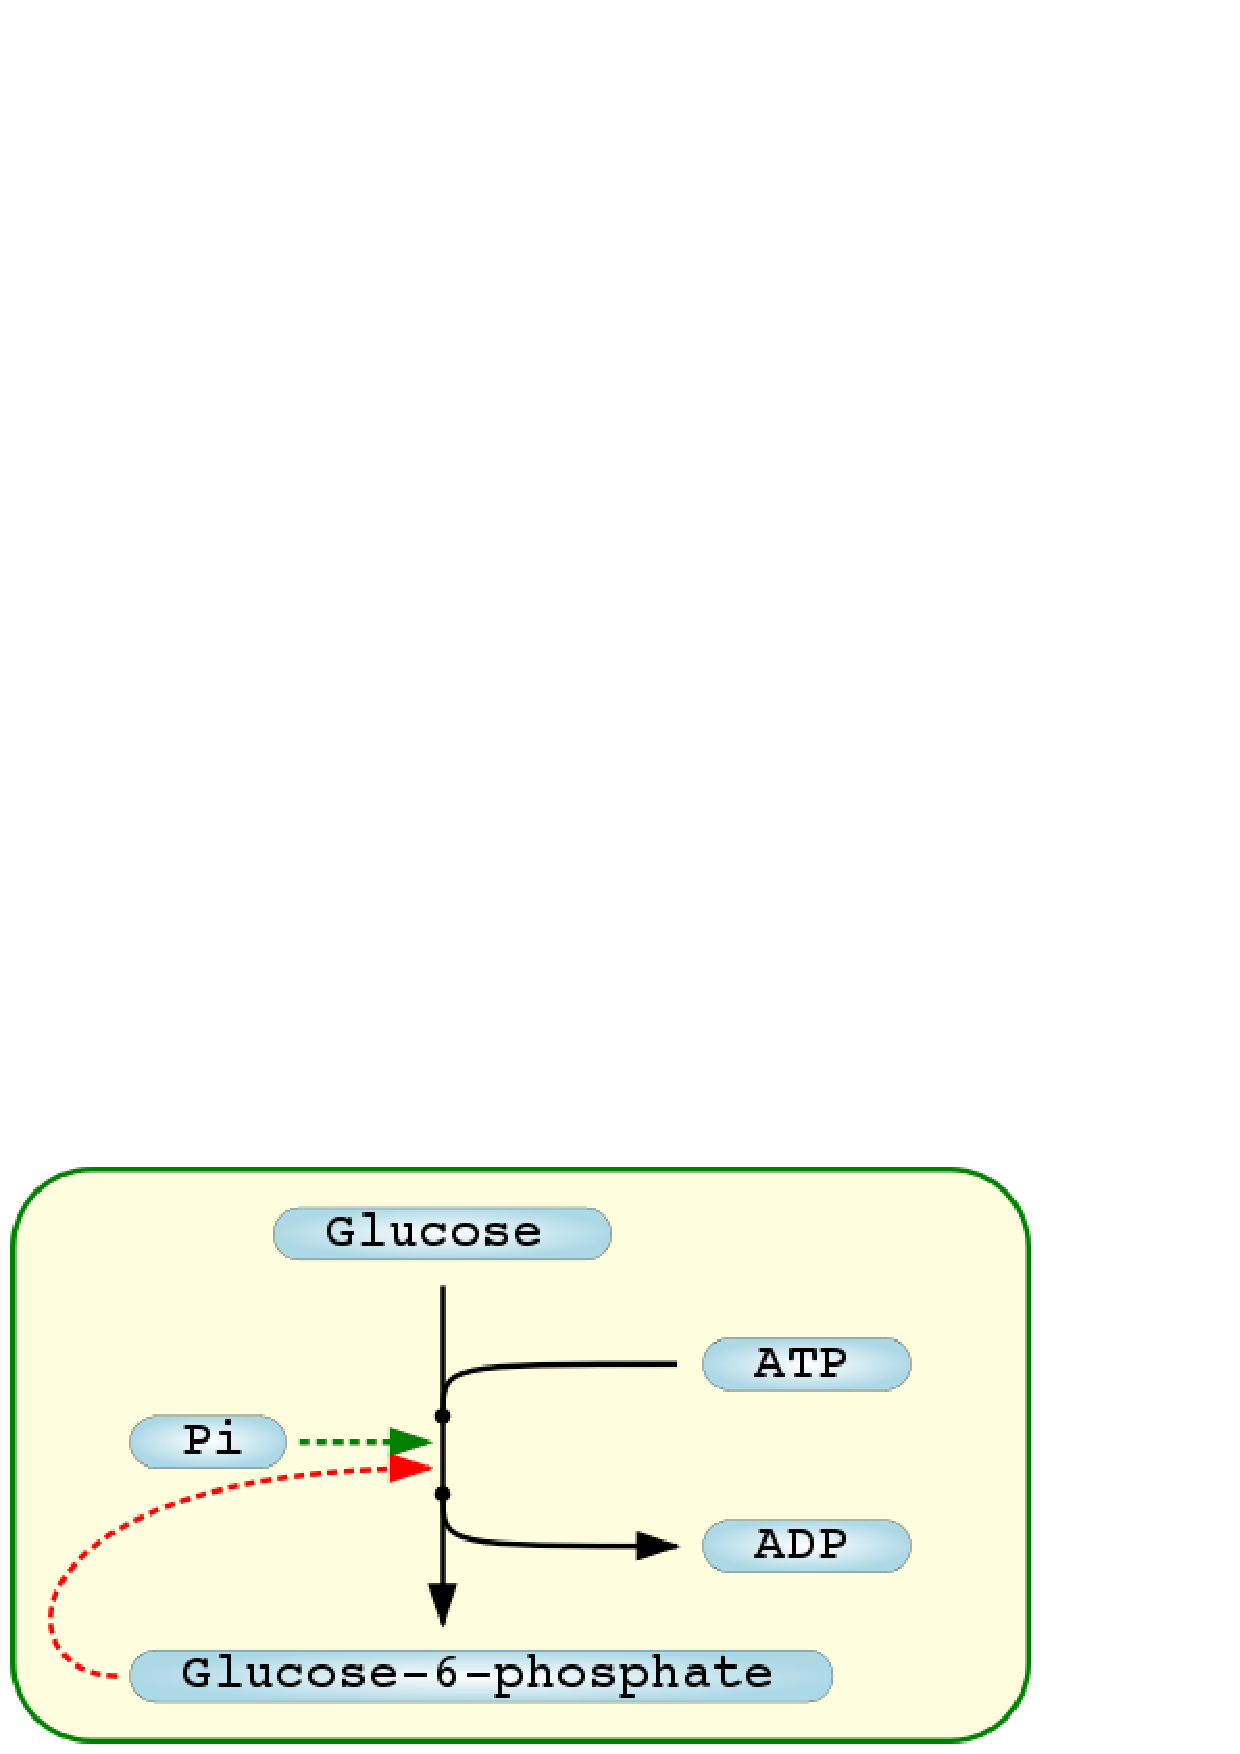
\includegraphics[scale=0.5]{figures/TestModel3-g++}
\caption{Another possible rendering of the example layout.}
\end{figure}
\end{center}

In order to use the Layout package in \SBML Level~2 documents, all that 
is needed is to use the Level 2 Namespace (see \ref{xml-namespace}) and 
move the \ListOfLayouts into the \Model \token{annotation} element. 



\begin{example}
<?xml version="1.0" encoding="UTF-8"?>
<sbml xmlns="http://www.sbml.org/sbml/level2" level="2" version="1">
  <model id="TestModel_with_modifiers">
    <annotation>
     <listOfLayouts xmlns="http://projects.eml.org/bcb/sbml/level2"
              xmlns:xsi="http://www.w3.org/2001/XMLSchema-instance">
      <layout id="Layout_1">
        <dimensions width="400" height="230"/>
        <listOfCompartmentGlyphs>
          <compartmentGlyph id="CompartmentGlyph_1" compartment="Yeast">
            <boundingBox id="bb1">
              <position x="5" y="5"/>
              <dimensions width="390" height="220"/>
            </boundingBox>
          </compartmentGlyph>
        </listOfCompartmentGlyphs>
        <listOfSpeciesGlyphs>
          <speciesGlyph id="SpeciesGlyph_Glucose" species="Glucose">
            <boundingBox id="bb2">
              <position x="105" y="20"/>
              <dimensions width="130" height="20"/>
            </boundingBox>
          </speciesGlyph>
          <speciesGlyph id="SpeciesGlyph_G6P" species="G6P">
            <boundingBox id="bb5">
              <position x="50" y="190"/>
              <dimensions width="270" height="20"/>
            </boundingBox>
          </speciesGlyph>
          <speciesGlyph id="SpeciesGlyph_ATP" species="ATP">
            <boundingBox id="bb3">
              <position x="270" y="70"/>
              <dimensions width="80" height="20"/>
            </boundingBox>
          </speciesGlyph>
          <speciesGlyph id="glyph_ADP" species="ADP">
            <boundingBox id="bb4">
              <position x="270" y="140"/>
              <dimensions width="80" height="20"/>
            </boundingBox>
          </speciesGlyph>
          <speciesGlyph id="SpeciesGlyph_Pi" species="Pi">
            <boundingBox id="bb6">
              <position x="50" y="100"/>
              <dimensions width="60" height="20"/>
            </boundingBox>
          </speciesGlyph>
        </listOfSpeciesGlyphs>
        <listOfReactionGlyphs>
          <reactionGlyph id="glyph_Hexokinase" reaction="Hexokinase">
            <curve>
              <listOfCurveSegments>
                <curveSegment xsi:type="LineSegment">
                  <start x="170" y="100"/>
                  <end x="170" y="130"/>
                </curveSegment>
              </listOfCurveSegments>
            </curve>
            <listOfSpeciesReferenceGlyphs>
              <speciesReferenceGlyph id="SpeciesReferenceGlyph_Glucose"
                            speciesReference="SpeciesReference_Glucose"
                            speciesGlyph="SpeciesGlyph_Glucose" role="substrate">
                <curve>
                  <listOfCurveSegments>
                    <curveSegment xsi:type="LineSegment">
                      <start x="170" y="100"/>
                      <end x="170" y="50"/>
                    </curveSegment>
                  </listOfCurveSegments>
                </curve>
              </speciesReferenceGlyph>
              <speciesReferenceGlyph id="SpeciesReferenceGlyph_ATP" 
                            speciesReference="SpeciesReference_ATP"
                            speciesGlyph="SpeciesGlyph_ATP" role="sidesubstrate">
                <curve>
                  <listOfCurveSegments>
                    <curveSegment xsi:type="CubicBezier">
                      <start x="170" y="100"/>
                      <end x="260" y="80"/>
                      <basePoint1 x="170" y="80"/>
                      <basePoint2 x="170" y="80"/>
                    </curveSegment>
                  </listOfCurveSegments>
                </curve>
              </speciesReferenceGlyph>
              <speciesReferenceGlyph id="SpeciesReferenceGlyph_G6P_1"
                              speciesReference="SpeciesReference_G6P"
                              speciesGlyph="SpeciesGlyph_G6P" role="product">
                <curve>
                  <listOfCurveSegments>
                    <curveSegment xsi:type="LineSegment">
                      <start x="170" y="130"/>
                      <end x="170" y="180"/>
                    </curveSegment>
                  </listOfCurveSegments>
                </curve>
              </speciesReferenceGlyph>
              <speciesReferenceGlyph id="SpeciesReferenceGlyph_ADP"
                            speciesReference="SpeciesReference_ADP"
                            speciesGlyph="glyph_ADP" role="sideproduct">
                <curve>
                  <listOfCurveSegments>
                    <curveSegment xsi:type="CubicBezier">
                      <start x="170" y="130"/>
                      <end x="260" y="150"/>
                      <basePoint1 x="170" y="150"/>
                      <basePoint2 x="170" y="150"/>
                    </curveSegment>
                  </listOfCurveSegments>
                </curve>
              </speciesReferenceGlyph>
              <speciesReferenceGlyph id="SpeciesReferenceGlyph_G6P_2"
                      speciesReference="ModifierSpeciesReference_G6P"
                      speciesGlyph="SpeciesGlyph_G6P" role="inhibitor">
                <curve>
                  <listOfCurveSegments>
                    <curveSegment xsi:type="CubicBezier">
                      <start x="45" y="200"/>
                      <end x="165" y="120"/>
                      <basePoint1 x="0" y="200"/>
                      <basePoint2 x="0" y="120"/>
                    </curveSegment>
                  </listOfCurveSegments>
                </curve>
              </speciesReferenceGlyph>
              <speciesReferenceGlyph id="SpeciesReferenceGlyph_PI"
                    speciesReference="ModifierSpeciesReference_Pi"
                    speciesGlyph="SpeciesGlyph_Pi" role="activator">
                <curve>
                  <listOfCurveSegments>
                    <curveSegment xsi:type="CubicBezier">
                      <start x="115" y="110"/>
                      <end x="165" y="110"/>
                      <basePoint1 x="140" y="110"/>
                      <basePoint2 x="140" y="110"/>
                    </curveSegment>
                  </listOfCurveSegments>
                </curve>
              </speciesReferenceGlyph>
            </listOfSpeciesReferenceGlyphs>
          </reactionGlyph>
        </listOfReactionGlyphs>
        <listOfTextGlyphs>
          <textGlyph id="TextGlyph_Glucose" graphicalObject="SpeciesGlyph_Glucose"
                     originOfText="Glucose">
            <boundingBox id="bbA">
              <position x="115" y="20"/>
              <dimensions width="110" height="20"/>
            </boundingBox>
          </textGlyph>
          <textGlyph id="TextGlyph_G6P" graphicalObject="SpeciesGlyph_G6P" 
                     originOfText="G6P">
            <boundingBox id="bbD">
              <position x="60" y="190"/>
              <dimensions width="250" height="20"/>
            </boundingBox>
          </textGlyph>
          <textGlyph id="TextGlyph_ATP" graphicalObject="SpeciesGlyph_ATP"
                     originOfText="ATP">
            <boundingBox id="bbB">
              <position x="280" y="70"/>
              <dimensions width="60" height="20"/>
            </boundingBox>
          </textGlyph>
          <textGlyph id="TextGlyph_ADP" graphicalObject="glyph_ADP"
                     originOfText="ADP">
            <boundingBox id="bbC">
              <position x="280" y="140"/>
              <dimensions width="60" height="20"/>
            </boundingBox>
          </textGlyph>
          <textGlyph id="TextGlyph_PI" graphicalObject="SpeciesGlyph_Pi"
                     originOfText="Pi">
            <boundingBox id="bbE">
              <position x="60" y="100"/>
              <dimensions width="40" height="20"/>
            </boundingBox>
          </textGlyph>
        </listOfTextGlyphs>
       </layout>
     </listOfLayouts>
    </annotation>
    <listOfCompartments>
      <compartment id="Yeast"/>
    </listOfCompartments>
    <listOfSpecies>
      <species id="Glucose" compartment="Yeast"/>
      <species id="G6P" name="Glucose-6-phosphate" compartment="Yeast"/>
      <species id="ATP" compartment="Yeast"/>
      <species id="ADP" compartment="Yeast"/>
      <species id="Pi" compartment="Yeast"/>
    </listOfSpecies>
    <listOfReactions>
      <reaction id="Hexokinase" reversible="false">
        <listOfReactants>
          <speciesReference species="Glucose">
            <annotation>
              <layoutId xmlns="http://projects.eml.org/bcb/sbml/level2"
                        id="SpeciesReference_Glucose"/>
            </annotation>
          </speciesReference>
          <speciesReference species="ATP">
            <annotation>
              <layoutId xmlns="http://projects.eml.org/bcb/sbml/level2" 
                        id="SpeciesReference_ATP"/>
            </annotation>
          </speciesReference>
        </listOfReactants>
        <listOfProducts>
          <speciesReference species="G6P">
            <annotation>
              <layoutId xmlns="http://projects.eml.org/bcb/sbml/level2" 
                        id="SpeciesReference_G6P"/>
            </annotation>
          </speciesReference>
          <speciesReference species="ADP">
            <annotation>
              <layoutId xmlns="http://projects.eml.org/bcb/sbml/level2"
                        id="SpeciesReference_ADP"/>
            </annotation>
          </speciesReference>
        </listOfProducts>
        <listOfModifiers>
          <modifierSpeciesReference species="G6P">
            <annotation>
              <layoutId xmlns="http://projects.eml.org/bcb/sbml/level2"
                        id="ModifierSpeciesReference_G6P"/>
            </annotation>
          </modifierSpeciesReference>
          <modifierSpeciesReference species="Pi">
            <annotation>
              <layoutId xmlns="http://projects.eml.org/bcb/sbml/level2" 
                        id="ModifierSpeciesReference_Pi"/>
            </annotation>
          </modifierSpeciesReference>
        </listOfModifiers>
      </reaction>
    </listOfReactions>
  </model>
</sbml>
\end{example}

\subsection{Example using the GeneralGlyph}
\label{example-generalglyph}
Here a small complete example that shows how to draw a basic influence
diagram, where \token{Node0} negatively influences \token{Node1}. 


\begin{center}
\begin{figure}[h!]
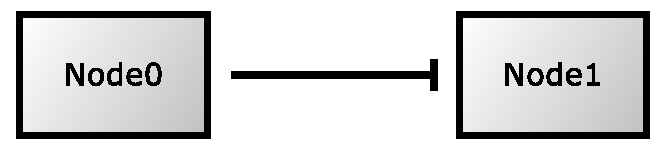
\includegraphics{figures/GeneralGlyphExample}
\caption{One possible rendering of an influence diagram.}
\end{figure}
\end{center}

In this example we have a simple SBML model that contains two species, 
\token{Node0} and \token{Node1}. For both of them there are species glyph
elements and associated Text labels. A \GeneralGlyph then represents the
influence. 

\exampleFile{xml/generalGlyph.sbml-l3v1.xml}

